\documentclass[11pt]{article}
%\renewcommand{\thesection}{\Roman{section}}  %zmiana section na rzymskie
\usepackage[utf8]{inputenc}
\usepackage[OT4]{polski}
\usepackage{tabularx}
\usepackage[margin=60pt]{geometry}
\usepackage{amsmath}
\usepackage{amsfonts}
\usepackage{listings} 
\usepackage[usenames,dvipsnames,table,xcdraw]{xcolor}
\usepackage{array}
\usepackage{sidecap} %do grafik
\usepackage{wrapfig} % j. w.
\usepackage{graphicx} %j.. w.
\usepackage{subfig} %j. w.
\usepackage{booktabs}
\usepackage{longtable}
\usepackage{hyperref}
\usepackage{nicefrac}
\usepackage{multirow}

\begin{document}
%%%%%%%%%%%%%%%%%%%%%%%%%%%%%%%%%%%%%%%%%%%%%%%%%%%%%%%%%%%%%%%%%%%%%%%%%%%%%%%
%%	tabelka
%%%%%%%%%%%%%%%%%%%%%%%%%%%%%%%%%%%%%%%%%%%%%%%%%%%%%%%%%%%%%%%%%%%%%%%%%%%%%%%%

\begin{table}[h!]
	\begin{tabular}{|l|l|l|ll|l|}	\hline
	\textbf{Laboratorium} & \multirow{2}{*}{ \textbf{\LARGE 6} } & \multicolumn{3}{l|}{\multirow{2}{*}{ \textbf{Podatność magnetyczna}} } &
	\multirow{3}*{\begin{tabular}{l} Zespół w składzie: \\ 1. Paweł Rzońca \\ 2. Paweł Kozioł \\ 3. Agata Sławska\end{tabular}  }\\
	\textbf{Fizyki Ciała Stałego} & & \multicolumn{3}{l|}{} &\\
	\cline{1-5}
	Wydział: \textbf{WFiIS} & \multicolumn{2}{l|}{Kierunek: \textbf{Fizyka Techniczna}} & Rok:& \textbf{3} & \\
	\cline{1-5}
	\multicolumn{2}{|l|}{Data wykonania: \textbf{5.11.2015} } & Data oddania: \textbf{19.11.2015} & Ocena:& &\\
	\hline
	\end{tabular}
\end{table}

%%%%%%%%%%%%%%%%%%%%%%%%%%%%%%%%%%%%%%%%%%%%%%%%%%%%%%%%%%%%%%%%%%%%%%%%%%%%%%%%


\section*{Aparatura i metodyka}
Aparatura użyta w ćwiczeniu:
\begin{itemize}
\item woltomierz fazoczuły
\item woltomierz do pośredniego pomiaru temperatury
\item układ pomiarowy z cewkami Helmholtza, grzałką oraz 
		układem do pomiaru temperatury
\item generator
\item próbki Ni, Gd$_2$O$_3$, Gd, TL-3, Dy oraz sonda 
\end{itemize}

Przed rozpoczęciem pomiaru odczekano na ustabilizowanie się woltomierza fazoczułego oraz zmierzono średnicę oraz ilość zwojów sondy.
Generator ustawiono na częstotliwość dla której wskazania woltomierza były największe. Następnie zmierzono wskazania tegoż woltomierza dla 
sondy i znaleziono maksimum. Następnie przystąpiono do pomiaru próbki Ni, gdzie rozpoczęto od miejsca gdzie wskazania były małe w porównaniu 
z tłem i odczytywano je co dwa obroty śruby mikrometrycznej. Pomiar zakończono, po uzyskaniu w przybliżeniu symetrycznej liczby pomiarów względem mierzonego 
maksimum. Pomiar powtórzono tenże pomiar dla Gd$_2$O$_3$ oraz dla Dy, tym razem skupiając się głównie na wyznaczeniu maksimum wskazania woltomierza. 
Następnie przygotowano układ do pomiaru podatności w funkcji temperatury dla półprzewodnika TL-3 orz Gd. 
W tym celu schłodzono układ wraz z próbką za pomocą ciekłego azotu i powoli podgrzewano go wbudowaną grzałką.
\section*{Opracowanie wyników}
\subsection*{A - Charakterystyka układu pomiarowego}
Wyniki pomiarów sondy:
$$d= 4 \mbox{ mm} \qquad N_H = 8.$$
Częstotliwość pracy generatora ustawiono na $f=160$ Hz. Przy tej częstotliwości otrzymano największe wskazanie $U_H = 56 $ mV.\\
Korzystając z prawa indukcji Faraday'a,
\begin{equation}
	U_H (t) = N_HSB_{0,\mbox{max}}\cos \omega t,
\end{equation}
Wyznaczono wartość $B_{0,\mbox{max}}$ pola magnesującego w układzie pomiarowym
\begin{equation}
	B_{0,\mbox{max}} = \frac{U_H \sqrt{2}}{N_HS\omega} = 0,8736 \mbox{ T,}
\end{equation}
gdzie $\omega=2\pi f$.

Następnie narysowano wykres (\ref{wyk_1}) zależności indukowanego napięcia w funkcji pozycji próbki Ni w układzie. Pomiar wykonano co dwa obroty śruby mikrometrycznej.

\begin{figure}[h!]
\centering
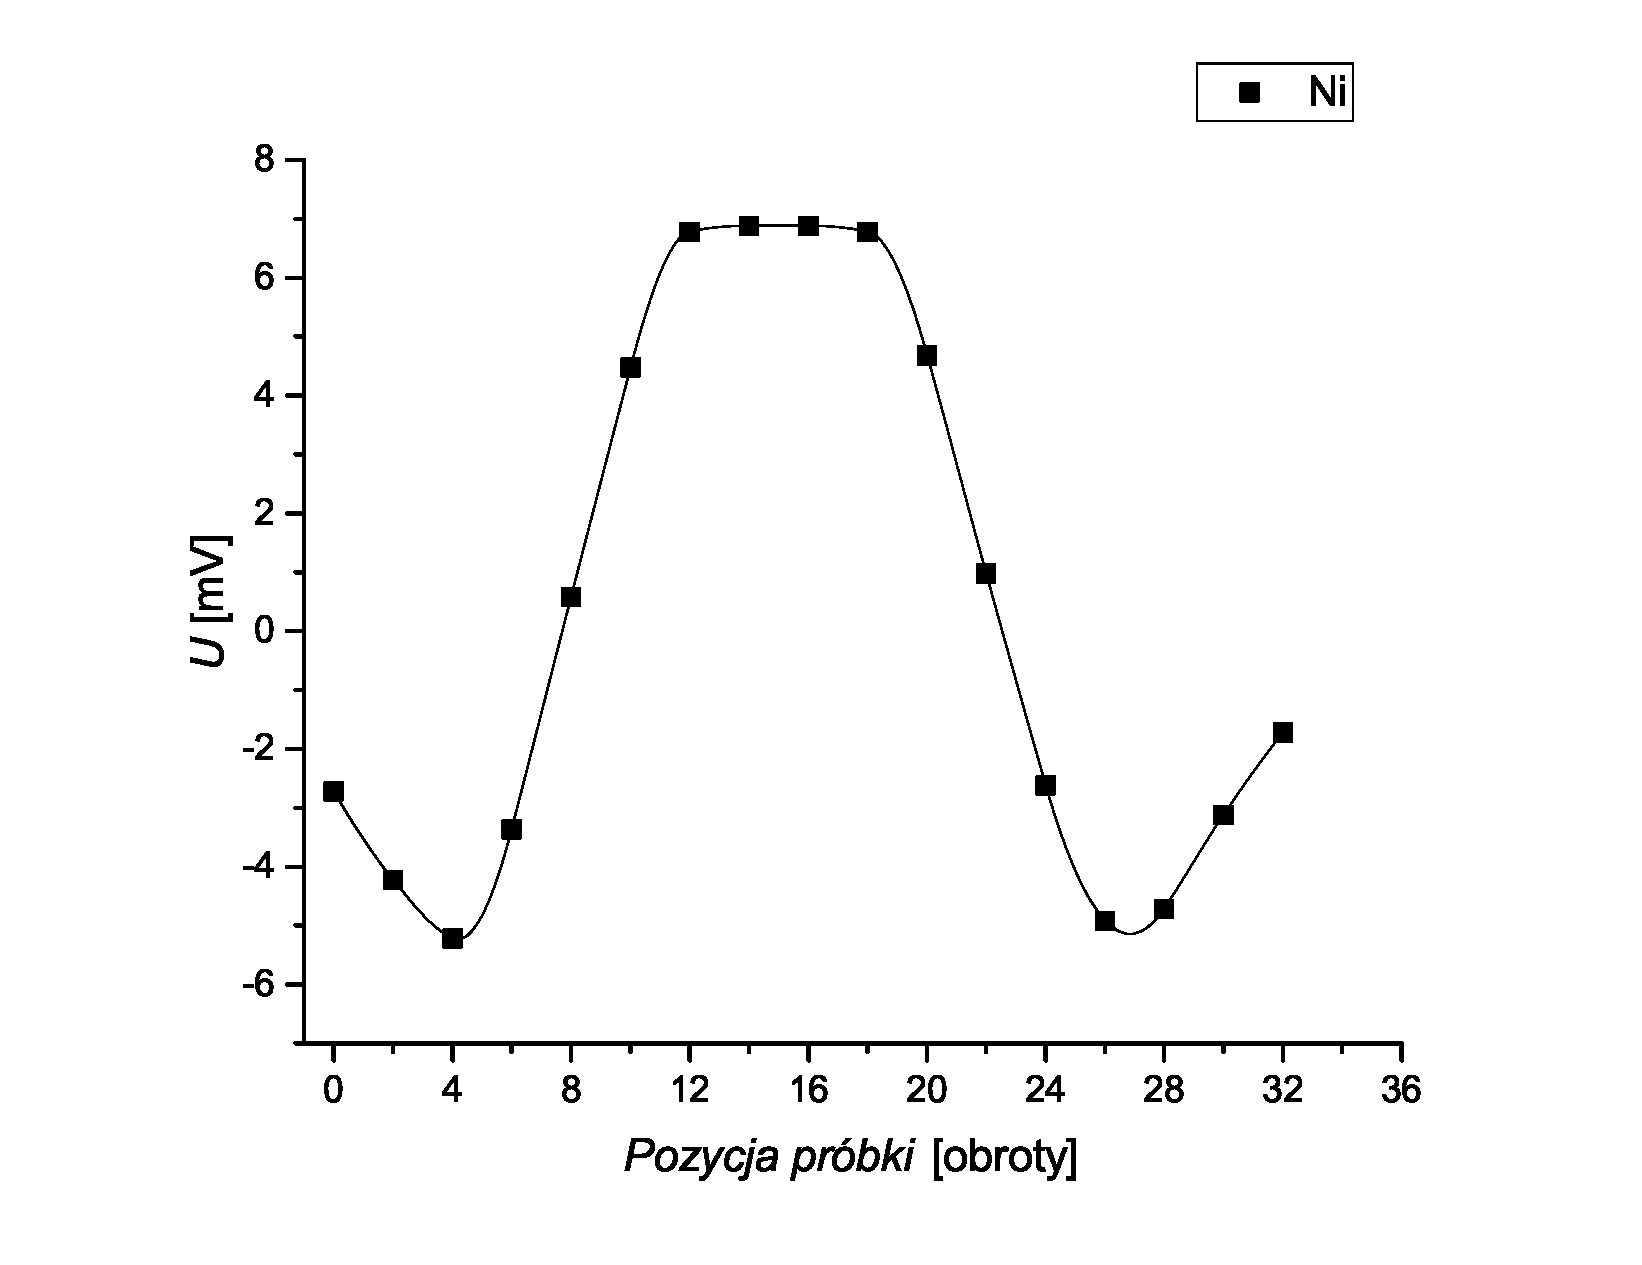
\includegraphics[width=0.8\textwidth]{./img/W1.eps}
\caption{Zależność indukowanego napięcia w funkcji pozycji próbki Ni w układzie detekcyjnym. Linię ciągłą dodano w programie Origin za pomocą 
funkcji dopasowującej gładką krzywą do wykresu i ma ona wyłącznie charakter poglądowy.}{\label{wyk_1}}
\end{figure}

\subsection*{B - Podatność magnetyczna}
W tabeli \ref{t1} zapisano wyniki pomiarów maksymalnego napięcia indukcji i tła oraz 
wyznaczonej podatności dla wybranych próbek, obliczonej przez porównanie do próbki wzorcowej 
przy użyciu zależności 

\begin{equation}
\frac{\chi_x m_x}{3V_{wz}} = \frac{U_{max,x}-U_{bg,x}}{U_{max,wz}-U_{bg,wz}}
\end{equation}

Za wzorcową przyjęto próbkę niklu. Dla tejże próbki:\\
$\begin{matrix}
	V_{kulki} = &160,3 & \mbox{[mg]} \\
	m_{kulki} = &18 & \mbox{[mm}^3] 
\end{matrix}$
\begin{equation}
\chi_{Ni} = 3\frac{V_{kulki}}{m_{kulki}} = 0,0003369 \left[ \frac{m^3}{kg} \right]
\end{equation}

\begin{table}[h!]
\centering
\caption{Wyniki pomiarów i obliczeń części B}{\label{t1}}
\begin{tabular}{|c|c|c|c|c|c|} \hline
\multirow{2}{*}{Próbka} & $m$ & $U_x$ & $U_{bg}$ & $\chi_{pomiar}$ & $\chi_{teoria}$ \\  
	& [mg] & [mV] & [mV] & [$\mu$m$^3$/kg]&[$\mu$m$^3$/kg] \\ \hline 
Gd$_2$O$_3$ & 216,5 & 25,8 & 22,0 & 1,38 & 1,74 \\ \hline
Dy & 82,2 & 8,77 & 7,90 & 8,31 & 7,55 \\ \hline
\end{tabular}
\end{table}

\subsection*{C - zależność podatności od temperatury}
Dla próbki Gd zmierzono indukowane napięcie w zależności od temperatury dla temperatur w zakresie (19-49) $^o$C. Od wyników odjęto zmierzone bezpośrednio przed
pomiarem tło $U_{bg}=23,7$ mV. Na wykresie \ref{ww2} przedstawiono zależność odwrotności indukowanego napięcia w funkcji temperatury. Napięcie to jest proporcjonalne
do podatności $\chi$. Do wykresu dopasowano prostą korzystając z programu Origin. Wartość, dla której przecina ona oś temperatur jest temperaturą Curie dla danej próbki Gd. 
$$ T_{Curie} = \frac{-b}{a} = 16,33\ ^o\mbox{C},$$
gdzie $a$ i $b$ to współczynniki dopasowania prostej $y=ax+b$, wynoszące odpowiednio
$$ a= 0,06791 [\mbox{1/mV}\cdot ^o\mbox{C}] \qquad b=-1.10916 [\mbox{1/mV}] $$
\begin{figure}[h!]
\centering
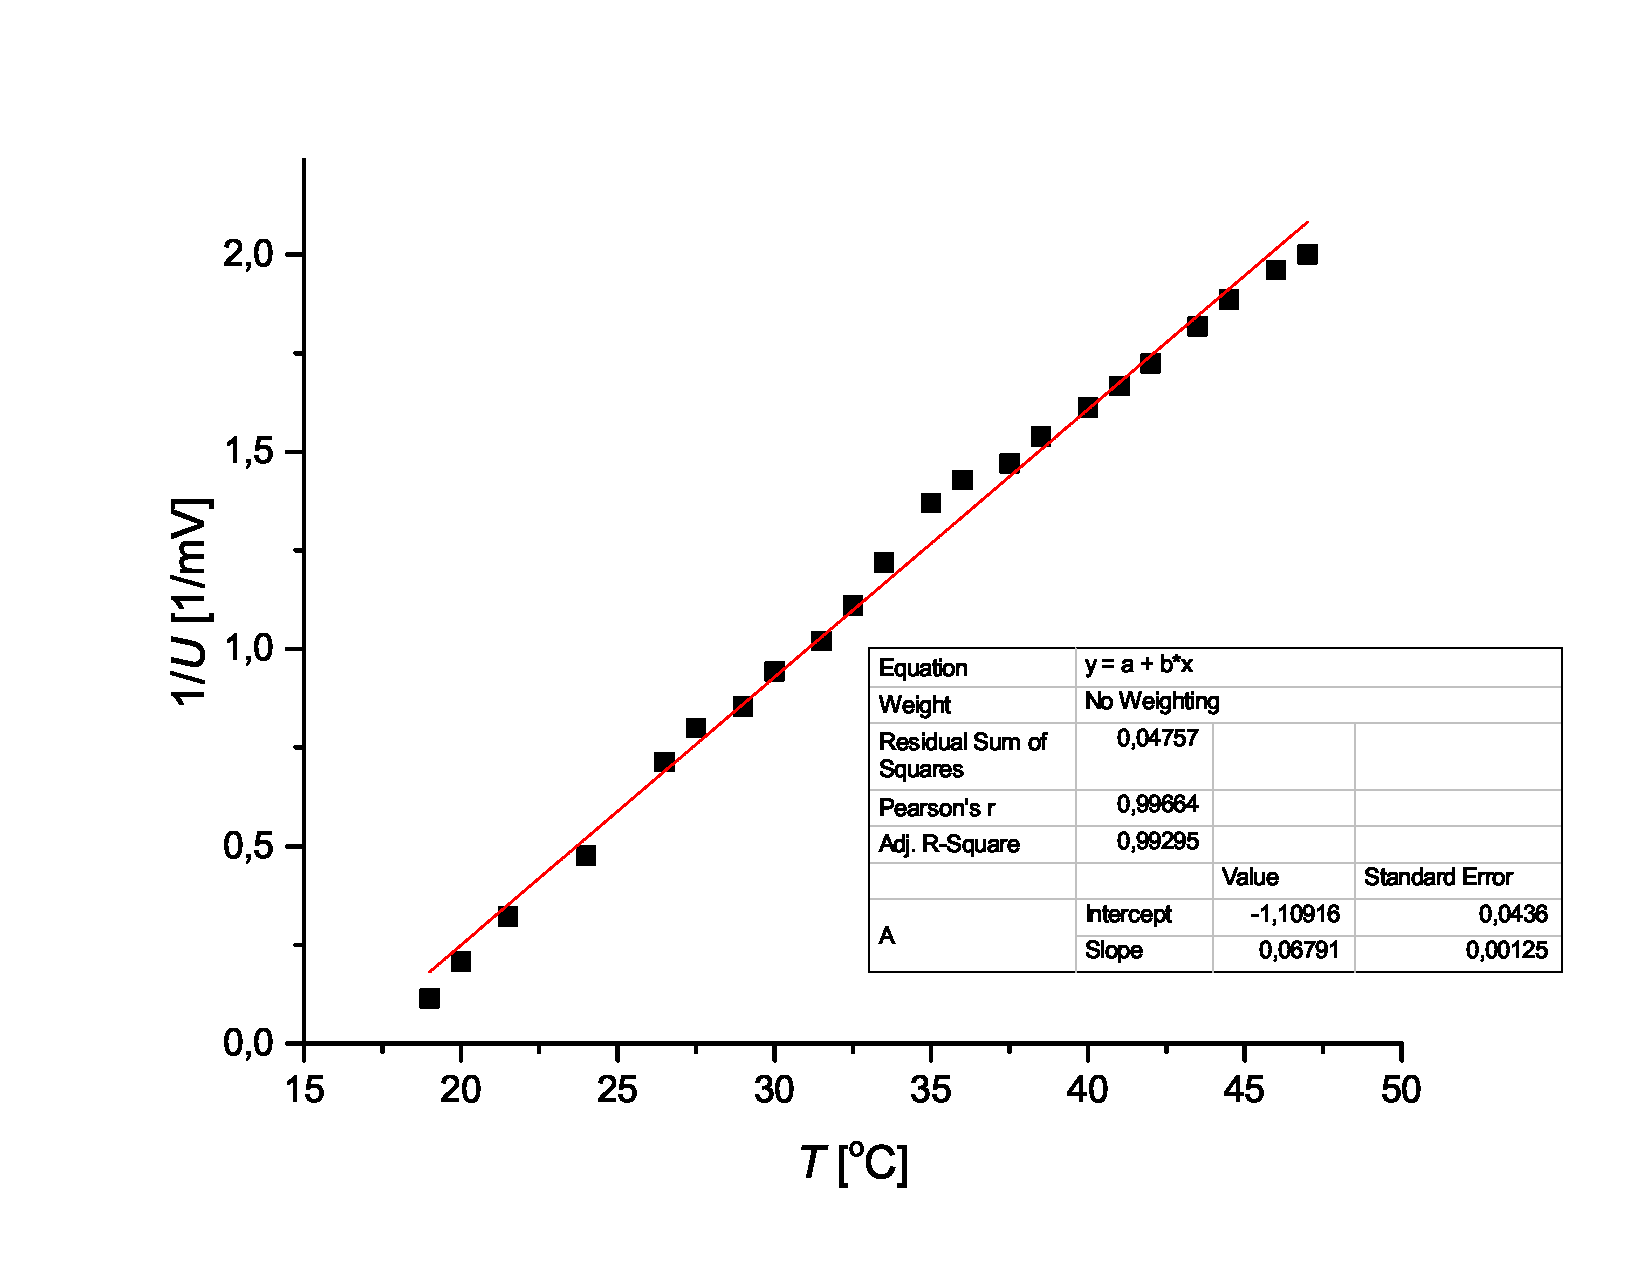
\includegraphics[width=0.8\textwidth]{./img/Gd.eps}
\caption{Zależność odwrotności indukowanego napięcia (odczyt po odjęciu tła) w zależności od temperatury dla próbki Gd.}{\label{ww2}}
\end{figure}

Pomiar dla próbki nadprzewodnika TL-3 wykonano zaczynając od temperatury wrzenia ciekłego azotu, a zakończono kilka punktów po gwałtownej zmianie, charakterystycznej 
dla nadprzewodników. Wyniki obliczeń podatności zebrano w tabeli \ref{3} oraz przedstawiono na wykresie \ref{wyk_3}. Zaobserwowano gwałtowny zanik podatności w okolicy -153 $^o$C co sugeruje, iż nastąpiło przejście fazowe w próbce. 
\begin{figure}[h!]
\centering
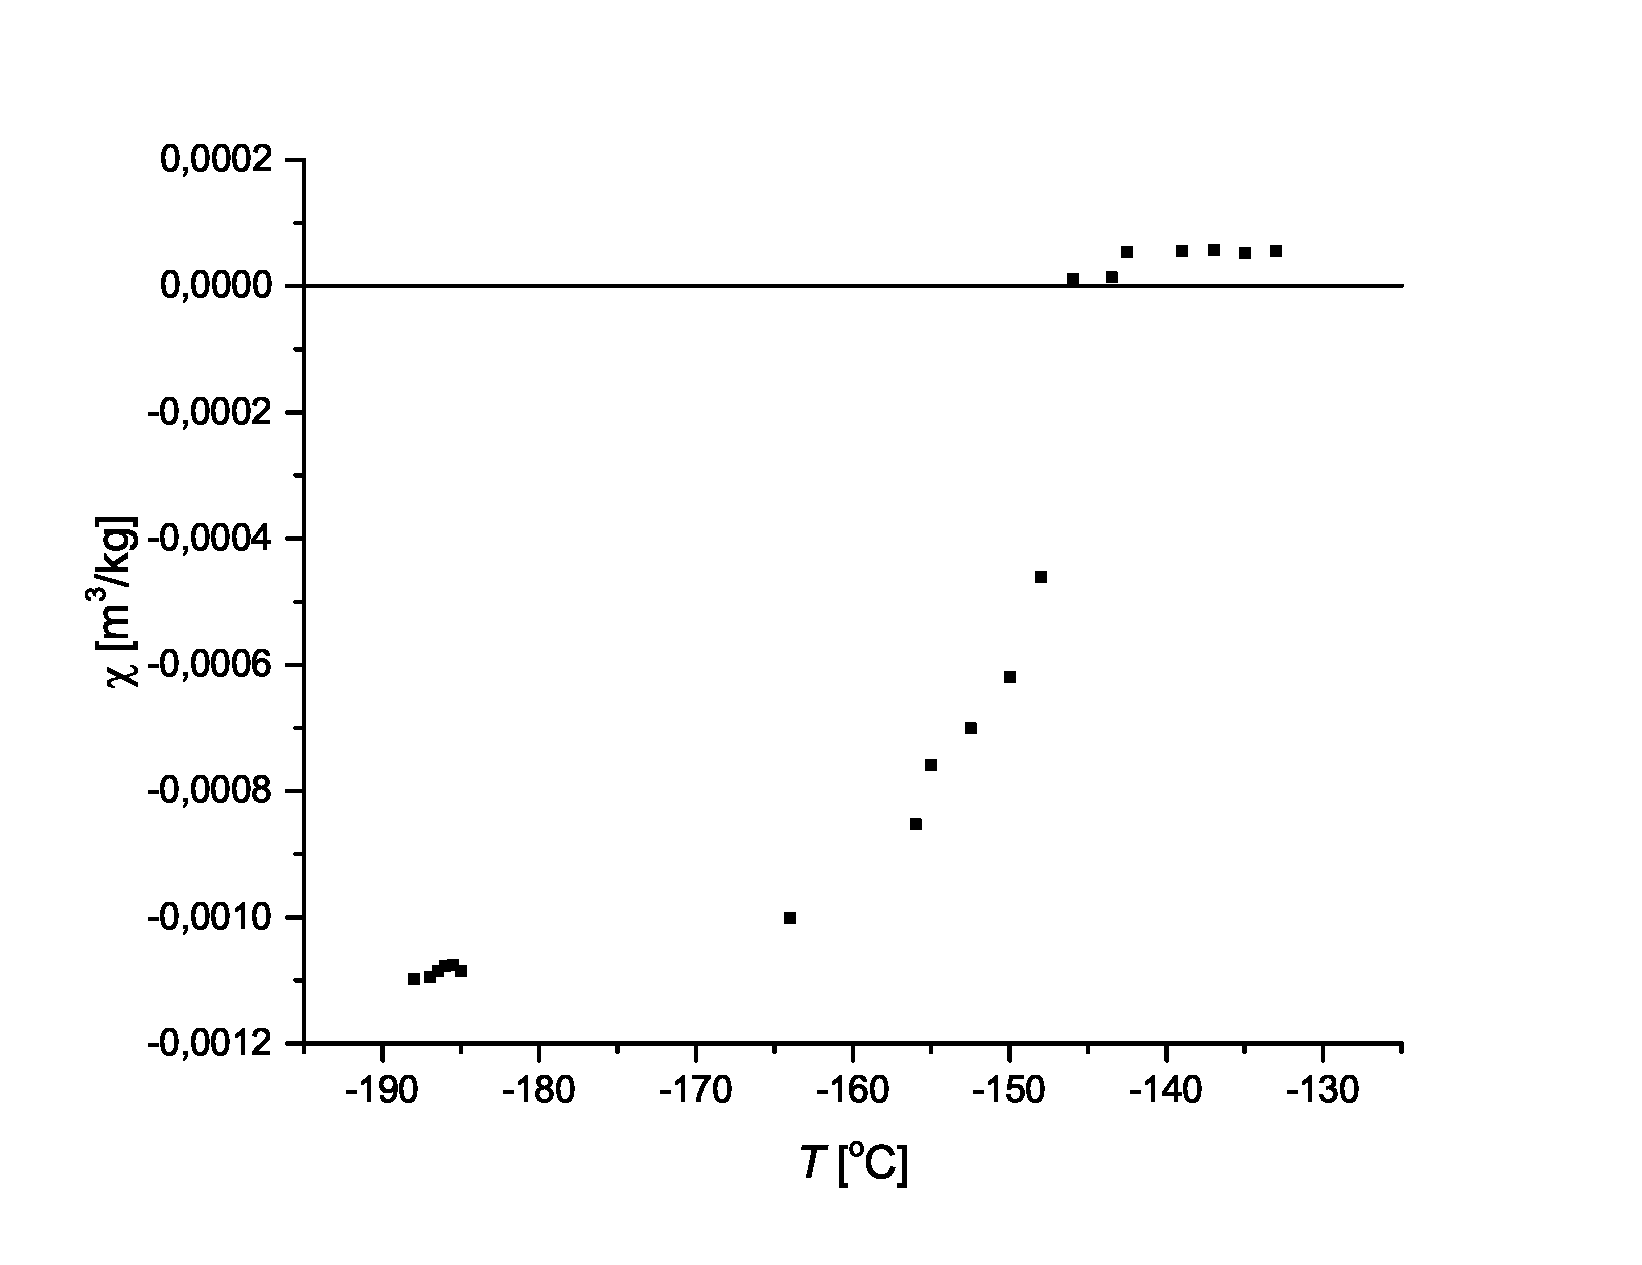
\includegraphics[width=0.8\textwidth]{./img/TL.eps}
\caption{Zależność indukowanego napięcia w funkcji pozycji próbki Ni w układzie detekcyjnym.}{\label{wyk_3}}
\end{figure}
\newpage
\section*{Podsumowanie}
W pierwszej części doświadczenia wyznaczono charakterystykę układu i przedstawiono ją na wykresie \ref{wyk_1}. Wynika ona z budowy układu, mianowicie 
z potrzeby ekranowania pola magnetycznego wytwarzanego bezpośrednio przez prąd z generatora w miejscu cewek miernika.

Następnie wyznaczono podatności magnetyczny próbek Gd$_2$O$_3$ oraz Dy:
\begin{center}\begin{tabular}{ccc}&$\chi_{pomiar}$ & $\chi_{teoria}$ \\  
&[$\mu$m$^3$/kg]&[$\mu$m$^3$/kg] \\
Gd$_2$O$_3$&1,38 & 1,74 \\ 
Dy & 8,31 & 7,55. \end{tabular}\end{center}
Wyznaczono również temperaturę Curie dla próbki gadolinu:
$$ T_{Curie,x} = 16,3\ [^o\mbox{C}] \qquad T_{Curie,tab} = 20\ [^o\mbox{C}]$$
oraz sporządzono wykres podatności w funkcji temperatury dla nadprzewodnika TL-3, na którym zaobserwowano przejście fazowe dla $T_{C} \approx -153\ ^o$C. 
Dla wyższych temperatur $\chi \approx 0 [\mbox{m}^3\mbox{/kg}]$, a dla niższych $\chi \approx 0,0011 [\mbox{m}^3\mbox{/kg}]$.

Porównując z wartościami tablicowymi (źr. $[$2$]$) wyniki można uznać za zadowalające. Mierzone wartości były bardzo małe, porównywalne z tłem. 
Jest to znaczne utrudnienie pomiaru i błędy mogą wynikać z niedokładności odczytu zarówno indukowanego napięcia jak i tła. 

\begin{thebibliography}{99}
%\bibitem{const} \url{http://const.physics.edu.pl/}
\bibitem{AGH} Łukasz Gondek, Marcin Sikora, Joanna Czub: \textit{Laboratorium Fizyki Fazy Skondenso-
wanej}, Wydawnictwa AGH, Kraków 2014
\bibitem{tablice} Tablice podatności magnetycznej $\chi$ dostępne [18.11.2015] pod linkiem 
\url{http://www.fizika.si/magnetism/MagSusceptibilities.pdf}
\bibitem{33} Opis ćwiczenia dostępny w laboratorium.
\end{thebibliography}


\section*{Aneks}
\begin{table}[h!]
\centering
\caption{Pomiary napięcia wskazywanego przez aparaturę w zależności od temperatury dla próbki Gd. Temperaturę przeliczono na $^o$C za pomocą tabeli
ze źródła [3].Gdzie napięcie $U_{bg}=23,7$ mV.}
\label{2}
\begin{tabular}{|l|l|}
\hline
$1 /(U_{x}-U_{bg})$ & $T$ \\  
$[$1/mV$]$ & $[ ^o$C$]$ \\ \hline
0,113 & 19,0 \\ \hline
0,208 & 20,0 \\ \hline
0,322 & 21,5 \\ \hline
0,476 & 24,0 \\ \hline
0,714 & 26,5 \\ \hline
0,800 & 27,5 \\ \hline
0,854 & 29,0 \\ \hline
0,943 & 30,0 \\ \hline
1,020 & 31,5 \\ \hline
1,111 & 32,5 \\ \hline
1,219 & 33,5 \\ \hline
1,369 & 35,0 \\ \hline
1,428 & 36,0 \\ \hline
1,470 & 37,5 \\ \hline
1,538 & 38,5 \\ \hline
1,612 & 40,0 \\ \hline
1,666 & 41,0 \\ \hline
1,724 & 42,0 \\ \hline
1,818 & 43,5 \\ \hline
1,886 & 44,5 \\ \hline
1,960 & 46,0 \\ \hline
2,000 & 47,0 \\ \hline
2,127 & 48,0 \\ \hline
2,173 & 49,0 \\ \hline
\end{tabular}
\end{table}
\begin{table}[h!]
\centering
\caption{Pomiary napięcia wskazywanego przez aparaturę w zależności od temperatury dla próbki TL-3. Temperaturę przeliczono na $^o$C za pomocą tabeli
ze źródła [2]}
\label{3}
\begin{tabular}{|l|l|}
\hline
$\chi$ & $T$ \\  
$[$m$^3$/kg$]$ & $[ ^o$C$]$ \\ \hline
-0,001098        & -188   \\ \hline
-0,001094        & -187   \\ \hline
-0,001086         & -186,5 \\ \hline
-0,001078        & -186   \\ \hline
-0,001075        & -185,5 \\ \hline
-0,001086         & -185   \\ \hline
-0,001002        & -164   \\ \hline
-0,0008526        & -156   \\ \hline
-0,0007591        & -155   \\ \hline
-0,0007007         & -152,5 \\ \hline
-0,0006190        & -150   \\ \hline
-0,0004613        & -148   \\ \hline
1,1679$\cdot 10^{-5}$ & -146   \\ \hline
1,4015$\cdot 10^{-5}$& -143,5 \\ \hline
5,3727$\cdot 10^{-5}$& -142,5 \\ \hline
5,4895$\cdot 10^{-5}$& -139   \\ \hline
5,7231$\cdot 10^{-5}$& -137   \\ \hline
5,2559$\cdot 10^{-5}$& -135   \\ \hline
5,4895$\cdot 10^{-5}$& -133   \\ \hline
\end{tabular}
\end{table}
\end{document}
